
\documentclass[journal,twoside]{IEEEtran}
\usepackage{lipsum}
\usepackage{fancyhdr}
\usepackage{ifpdf}
\usepackage{graphicx}
\usepackage{float}

\usepackage{makecell}
\usepackage[table]{xcolor}
\usepackage{xcolor, colortbl}	
\usepackage{amsmath}
\usepackage{amsfonts}
\usepackage{hyperref}
\usepackage{multirow}


\ifCLASSINFOpdf
\else
\fi


\makeatletter

\newcommand{\shortname}{Final Report} \def\ps@headings{
\def\@evenhead{\scriptsize\mbox{\MakeUppercase{\shortname}}\rightmark \hfil \thepage}\def\@oddhead{\scriptsize\thepage \hfil \leftmark\mbox{\MakeUppercase{\shortname}}}\def\@oddfoot{}\def\@evenfoot{}}\def\ps@IEEEtitlepagestyle{\def\@evenhead{\scriptsize\mbox{\MakeUppercase{\shortname}}\rightmark \hfil \thepage}\def\@oddhead{\scriptsize\thepage \hfil \leftmark\mbox{\MakeUppercase{\shortname}}}\def\@oddfoot{}\def\@evenfoot{}}\makeatother\pagestyle{headings}\pagenumbering{gobble}

\begin{document}

\title{Determining the state of thexas hold 'em in almost to real time}

\author{ David Molin\IEEEauthorrefmark{2} 
, 
Tomas Rosin Forsyth \IEEEauthorrefmark{8}

\IEEEcompsocitemizethanks{\IEEEcompsocthanksitem \IEEEauthorrefmark{2}dmolin@stanford.edu

\IEEEcompsocthanksitem \IEEEauthorrefmark{8}tomfo@stanford.edu}}% <-this % stops a space

\maketitle

\begin{abstract}
TODO

\end{abstract}

%\begin{IEEEkeywords}

%\end{IEEEkeywords}


\IEEEpeerreviewmaketitle


%%%%%%%%%%%%%%%%%%%%%%%%%%%%%%
%%%%%%%%%%  Introduction %%%%%%%%%%%%%%
%%%%%%%%%%%%%%%%%%%%%%%%%%%%%%

\section{Introduction}
The problem of automatically detecting suit and rank of playing cards based on a stream of images could potentially be used for  several commerical or non-commerical applications. One such application could be to automatically determine the cards on the table for broadcasting live poker tournaments.
Generally when attempting to match objects with a known template in images it is possible to use keypoint detectors such as SIFT \cite{SIFT} or ORB \cite{ORB} and match these keypoints and doing a geometric consistency check through the use of RANSAC. However due to the fact that the keypoints on poker cards would correspond to the corners of the suit symbols (check expression TODO) the ratio test described in \cite{SIFT} would reject most of the matches as there are multiple of each suit symbol on each card. TODO

%%%%%%%%%%%%%%%%%%%%%%%%%%%%%%
%%%%%%%%%%  Prior work %%%%%%%%%%%%%%
%%%%%%%%%%%%%%%%%%%%%%%%%%%%%%

\section{Prior work}

Some prior work has been done in this field for example \cite{PokerVision} uses optical character recognition in order to determine the 
TODO

%%%%%%%%%%%%%%%%%%%%%%%%%%%%%%
%%%%%%%%%%  Method %%%%%%%%%%%%%%%%
%%%%%%%%%%%%%%%%%%%%%%%%%%%%%%

\section{Method}

\begin{figure}[placement h]
\centering
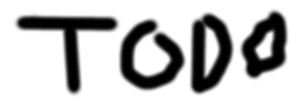
\includegraphics[scale=0.4, trim= 0cm 0cm 0cm 0cm]{TODO.png}
\caption{Outline of the process used for detecting cards in this paper}
\label{fig:AlgOutline}
\end{figure}

The process used in this paper for extracting the suit and rank of all cards in an image can be divided into two parts. The first part is extracting position of the corners of all cards and then from this position extract a image of the card oriented in a upright position with a known size. The other prat of the algorithm is to find the suit and rank from a image of a card placed in a upright position.

\subsection{Extracting the card corners}

\begin{figure}[placement h]
\centering
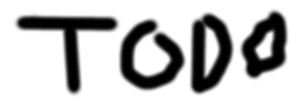
\includegraphics[scale=0.4, trim= 0cm 0cm 0cm 0cm]{TODO.png}
\caption{Pipeline for identifying the cards and finding their corners}
\label{fig:CornerOutline}
\end{figure}

First the assumption that the cards are considerably brighter than the background is made. This is usually true since poker cards are pieces of white paper and the table which poker is played on a green tablecloth, or in some cases on a wooden table.
This motivates why it should be possible to extract the poker cards from the background by using Otsu's method\cite{OTSU}.

Once Otsu's method has extracted a mask of the cards it is possible to extract the contours of the card by applying the method described in \cite{CONTOURS}. A card will have a contour consisting of 4 lines. Since playing cards are small and the distance to the playing cards are much larger than the size of the card there will be pairs of almost paralell lines for the contours of the cards. This stucture can be used by finding the paralell lines by using a Hough transform. In practice the hough transform is too slow for almost real time applications, therefore the progressive probabilistic hough transform described in \cite{HoughP}, This will give results similar to the one in the original Hough transform, but using less computation. From the hough transform it is possible to find the endpoints of long paralell lines. These points will usually correspond to the corners of the cards, some false positives might result from this but these can then be rejected at a later stage in the pipeline.

Once these corners are found it is trivial to find and apply an projective transformation whch maps the cards to a default size.

\subsection{Finding rank and suit of a card}

\begin{figure}[placement h]
\centering
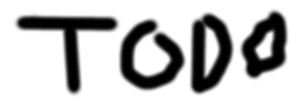
\includegraphics[scale=0.4, trim= 0cm 0cm 0cm 0cm]{TODO.png}
\caption{Pipeline for determining the rank and suit of a card}
\label{fig:RankSuitOutline}
\end{figure}

The color of the card can be extracted by comparing the red channel with some other color channel. For red cards such as diamonds and hearts the red channel will assume large values at all points on the card, this will not however be the case for black cards such as spades or clubs. This fact can then be used to determine if the suit of a card is red or black.

Since all cards have the suit symbol in the upper left corner it is possible to extract the suit by doing template matching in this region.

Furthermore it is possible to notice that the appearence of the face cards and nonface cards are quite different, the face cards consist of a large image suggesting that keypoint matching such as ORB or SIFT could be used to match these cards by comparing the extracted keypoints to the query card. This suggests that it should be a good idea to compute the rank for face cards and nonface cards in different ways.

In order to determine wheather a card is a face card or a nonface card the fact that face cards consist of one large connected blob, while nonface cards consist of several small blobs is used. Blobs are found by using Otsu's method. Then the size of the largest blob in the image is found. If this size is larger than some predetermined threshhold the image is classified as a face card.

When doing keypoint matching for the face cards some issues might arise for the ratio test in \cite{SIFT} since the bottom half of a face cards is a mirrored copy of the top half and therefore each feature would have a corresponding feature from the mirrored part of the card. This should however not be too much of an issue even if ignored and can be solved by instead of using the third closest feature for the ratio test instead of the second  closes feature. 

For nonface cards keypoints mathcing would be unsuitable due to the fact that keypoints would mainly be found for the suit symbols and these occur several times on each card and therefore the mathes would not be good.
Instead it is possbile to count the number of blobs on each nonface card. Each blob will correspond to one suit symbol. In order to supress noise the blobs would have to be larger than a given threshhold, otherwise the small symbols in the corner of the cards as well as small blobs created by noise would contribute to the rank of the card. The blobs are found by applying otsu's method on the blue channel of the cards.

%%%%%%%%%%%%%%%%%%%%%%%%%%%%%%
%%%%%%%%%%  Results %%%%%%%%%%%%%%%%
%%%%%%%%%%%%%%%%%%%%%%%%%%%%%%
\section{Results}

\subsection{Test set}

IMAGES OF THE TEST SET TODO

The method for determining the suit and rank of the cards described in method is in this section applied to a test set of 20 images, each containing 3 cards taken in an indoor environment with conditions similar to the ones for a real pokertable. In other words clutter will be present and the images will not be close ups of poker cards taken from above. Some photographs will include motion blur as this will generally be present when a mobile device is used for determining cards in real time.

\begin{table}[placement h]
    \label{tab:Confusion}
    \centering

\begin{tabular}{cc|c|l|l|}
\cline{3-4}
& & \multicolumn{2}{ c| }{Real class} \\ \cline{3-4}
& & Card & Non card  \\ \cline{1-4}
\multicolumn{1}{ |c| }{\multirow{2}{*}{Detected class} } &
\multicolumn{1}{ |c| }{Card} & 54 & 0     \\ \cline{2-4}
\multicolumn{1}{ |c  }{}                        &
\multicolumn{1}{ |c| }{NonCard} & 6 & -    \\ \cline{1-4}
\end{tabular} \\

\caption{Confusion matrix of the cards detected by the algorithm}

\end{table}

The confusion matrix shows that the results for detecting the cards is good.

using the method described earlier on the test set the accuracy for suit detection is $83\%$ for all of the detected cards. The main problem in suit detection seems to be that clubs are detected as spaces, This happened in 7 out of the 9 cases where the suit was incorrectly detected. The correct rank is detected for $92.5\%$ of the detected cards. The detected rank was usually off by one to the correct rank of the card. The accuracy of the whole pipeline is $66\%$

CARDS $\&$ IMAGES INCorectly CLASSIFIED IMAGES

COMMENTS ON the incorrectly classified images

CARDS $\&$ IMAGES Corectly CLASSIFIED IMAGES

COMMENTS ON the correctly classified images

TODO

%%%%%%%%%%%%%%%%%%%%%%%%%%%%%%
%%%%%%%%%%  Discussion %%%%%%%%%%%%%%%%
%%%%%%%%%%%%%%%%%%%%%%%%%%%%%%

\section{Discussion}

As can be seen in the results section this approach gives pretty good results. Although they are slightly worse than the results in \cite{PokerVision} which had a accuracy of $93\%$, however it is hard to compare these results directly since this paper did not use the same test set as\cite{PokerVision}. In order to be able to use a card detector in practice it should have a accuracy which is $>98\%$. For lower accuracies than this errors will be so common that it is neccesary to have a human for correcting the error of the card analyzer.
Although the error of this approach is too high for practical applications it might be possible to improve the results to an acceptable rate by increasing the accuracy of the corners detection step in the algorithm and the template matching step.

%%%%%%%%%%%%%%%%%%%%%%%%%%%%%%
%%%%%%%%%%  Future work %%%%%%%%%%%%%%%%
%%%%%%%%%%%%%%%%%%%%%%%%%%%%%%

\subsection{Future work}

Future work could include to find a way to make this method work with occluded cards and for cases where the cards are placed on top of each other. It should also be possible to improve the results by making a better corner detector as the corners are not perfectly detected by the current pipeline which means that the recognition step gets a slightly warped card as an input. One of the major reasons for why the suit detection was bad was that clubs was often identified as spades and if a better method for discriminating inbetween spades and clubs the results would improve significantly. Since the cards used in the test set were reflective some cards in the test set had specular highlights, this problem is similar to occusion since it was not possible to determine the actual colors of the cards at these points.


%%%%%%%%%%%%%%%%%%%%%%%%%%%%%%
%%%%%%%%%%  Conclusion %%%%%%%%%%%%%%%%
%%%%%%%%%%%%%%%%%%%%%%%%%%%%%%

\section{Conclusion}




\begin{thebibliography}{9}

\bibitem{SIFT}
Lowe, David G. "Distinctive image features from scale-invariant keypoints." International journal of computer vision 60.2 (2004): 91-110.

\bibitem{ORB}
Rublee, Ethan, et al. "ORB: an efficient alternative to SIFT or SURF." Computer Vision (ICCV), 2011 IEEE International Conference on. IEEE, 2011.

\bibitem{PokerVision}
Martins, Paulo, Luís Paulo Reis, and Luís Teófilo. "Poker vision: playing cards and chips identification based on image processing." Pattern Recognition and Image Analysis. Springer Berlin Heidelberg, 2011. 436-443.

\bibitem{HoughP}
Matas, Jiri, Charles Galambos, and Josef Kittler. "Robust detection of lines using the progressive probabilistic hough transform." Computer Vision and Image Understanding 78.1 (2000): 119-137.

\bibitem{OTSU}
Otsu, Nobuyuki. "A threshold selection method from gray-level histograms." Automatica 11.285-296 (1975): 23-27.

\bibitem{CONTOURS}
Suzuki, Satoshi. "Topological structural analysis of digitized binary images by border following." Computer Vision, Graphics, and Image Processing 30.1 (1985): 32-46.

\bibitem{HoughP}
Matas, Jiri, Charles Galambos, and Josef Kittler. "Robust detection of lines using the progressive probabilistic hough transform." Computer Vision and Image Understanding 78.1 (2000): 119-137.


\bibliographystyle{IEEEtran}

\end{thebibliography}
\end{document}
